\documentclass{article} % For LaTeX2e
\usepackage{nips15submit_e,times}
\usepackage{hyperref}
\usepackage{url}
\usepackage{graphicx}
\graphicspath{ {/Users/Tyler/LOVEFest/Figures/pdf/} }
%\documentstyle[nips14submit_09,times,art10]{article} % For LaTeX 2.09


\title{Randomer Forests}


\author{
Tyler M. Tomita\thanks{ Use footnote for providing further information
about author (webpage, alternative address)---\emph{not} for acknowledging
funding agencies.} \\
Department of Biomedical Engineering\\
Johns Hopkins University\\
Baltimore, MD \\
\texttt{ttomita@jhu.edu} \\
\And
Joshua T. Vogelstein \\
Department of Biomedical Engineering \\
Johns Hopkins University \\
\texttt{email} \\
\AND
Coauthor \\
Affiliation \\
Address \\
\texttt{email} \\
\And
Coauthor \\
Affiliation \\
Address \\
\texttt{email} \\
\And
Coauthor \\
Affiliation \\
Address \\
\texttt{email} \\
(if needed)\\
}

% The \author macro works with any number of authors. There are two commands
% used to separate the names and addresses of multiple authors: \And and \AND.
%
% Using \And between authors leaves it to \LaTeX{} to determine where to break
% the lines. Using \AND forces a linebreak at that point. So, if \LaTeX{}
% puts 3 of 4 authors names on the first line, and the last on the second
% line, try using \AND instead of \And before the third author name.

\newcommand{\fix}{\marginpar{FIX}}
\newcommand{\new}{\marginpar{NEW}}

%\nipsfinalcopy % Uncomment for camera-ready version

\begin{document}

\maketitle

\begin{abstract}
Insert abstract
\end{abstract}

%\section{}

\begin{figure}[h]
\begin{center}
%\framebox[4.0in]{$\;$}
\includegraphics[trim=0in 7in 0in 7in, clip=true, width=0.8\linewidth]{Fig1_Lhat}
\end{center}
\caption{}
\end{figure}

\begin{figure}[h]
\begin{center}
%\framebox[4.0in]{$\;$}
\includegraphics[trim=0in 8.75in 0in 8.75in, clip=true, width=0.8\linewidth]{Fig2_Time}
\end{center}
\caption{}
\end{figure}

\begin{figure}[h]
\begin{center}
%\framebox[4.0in]{$\;$}
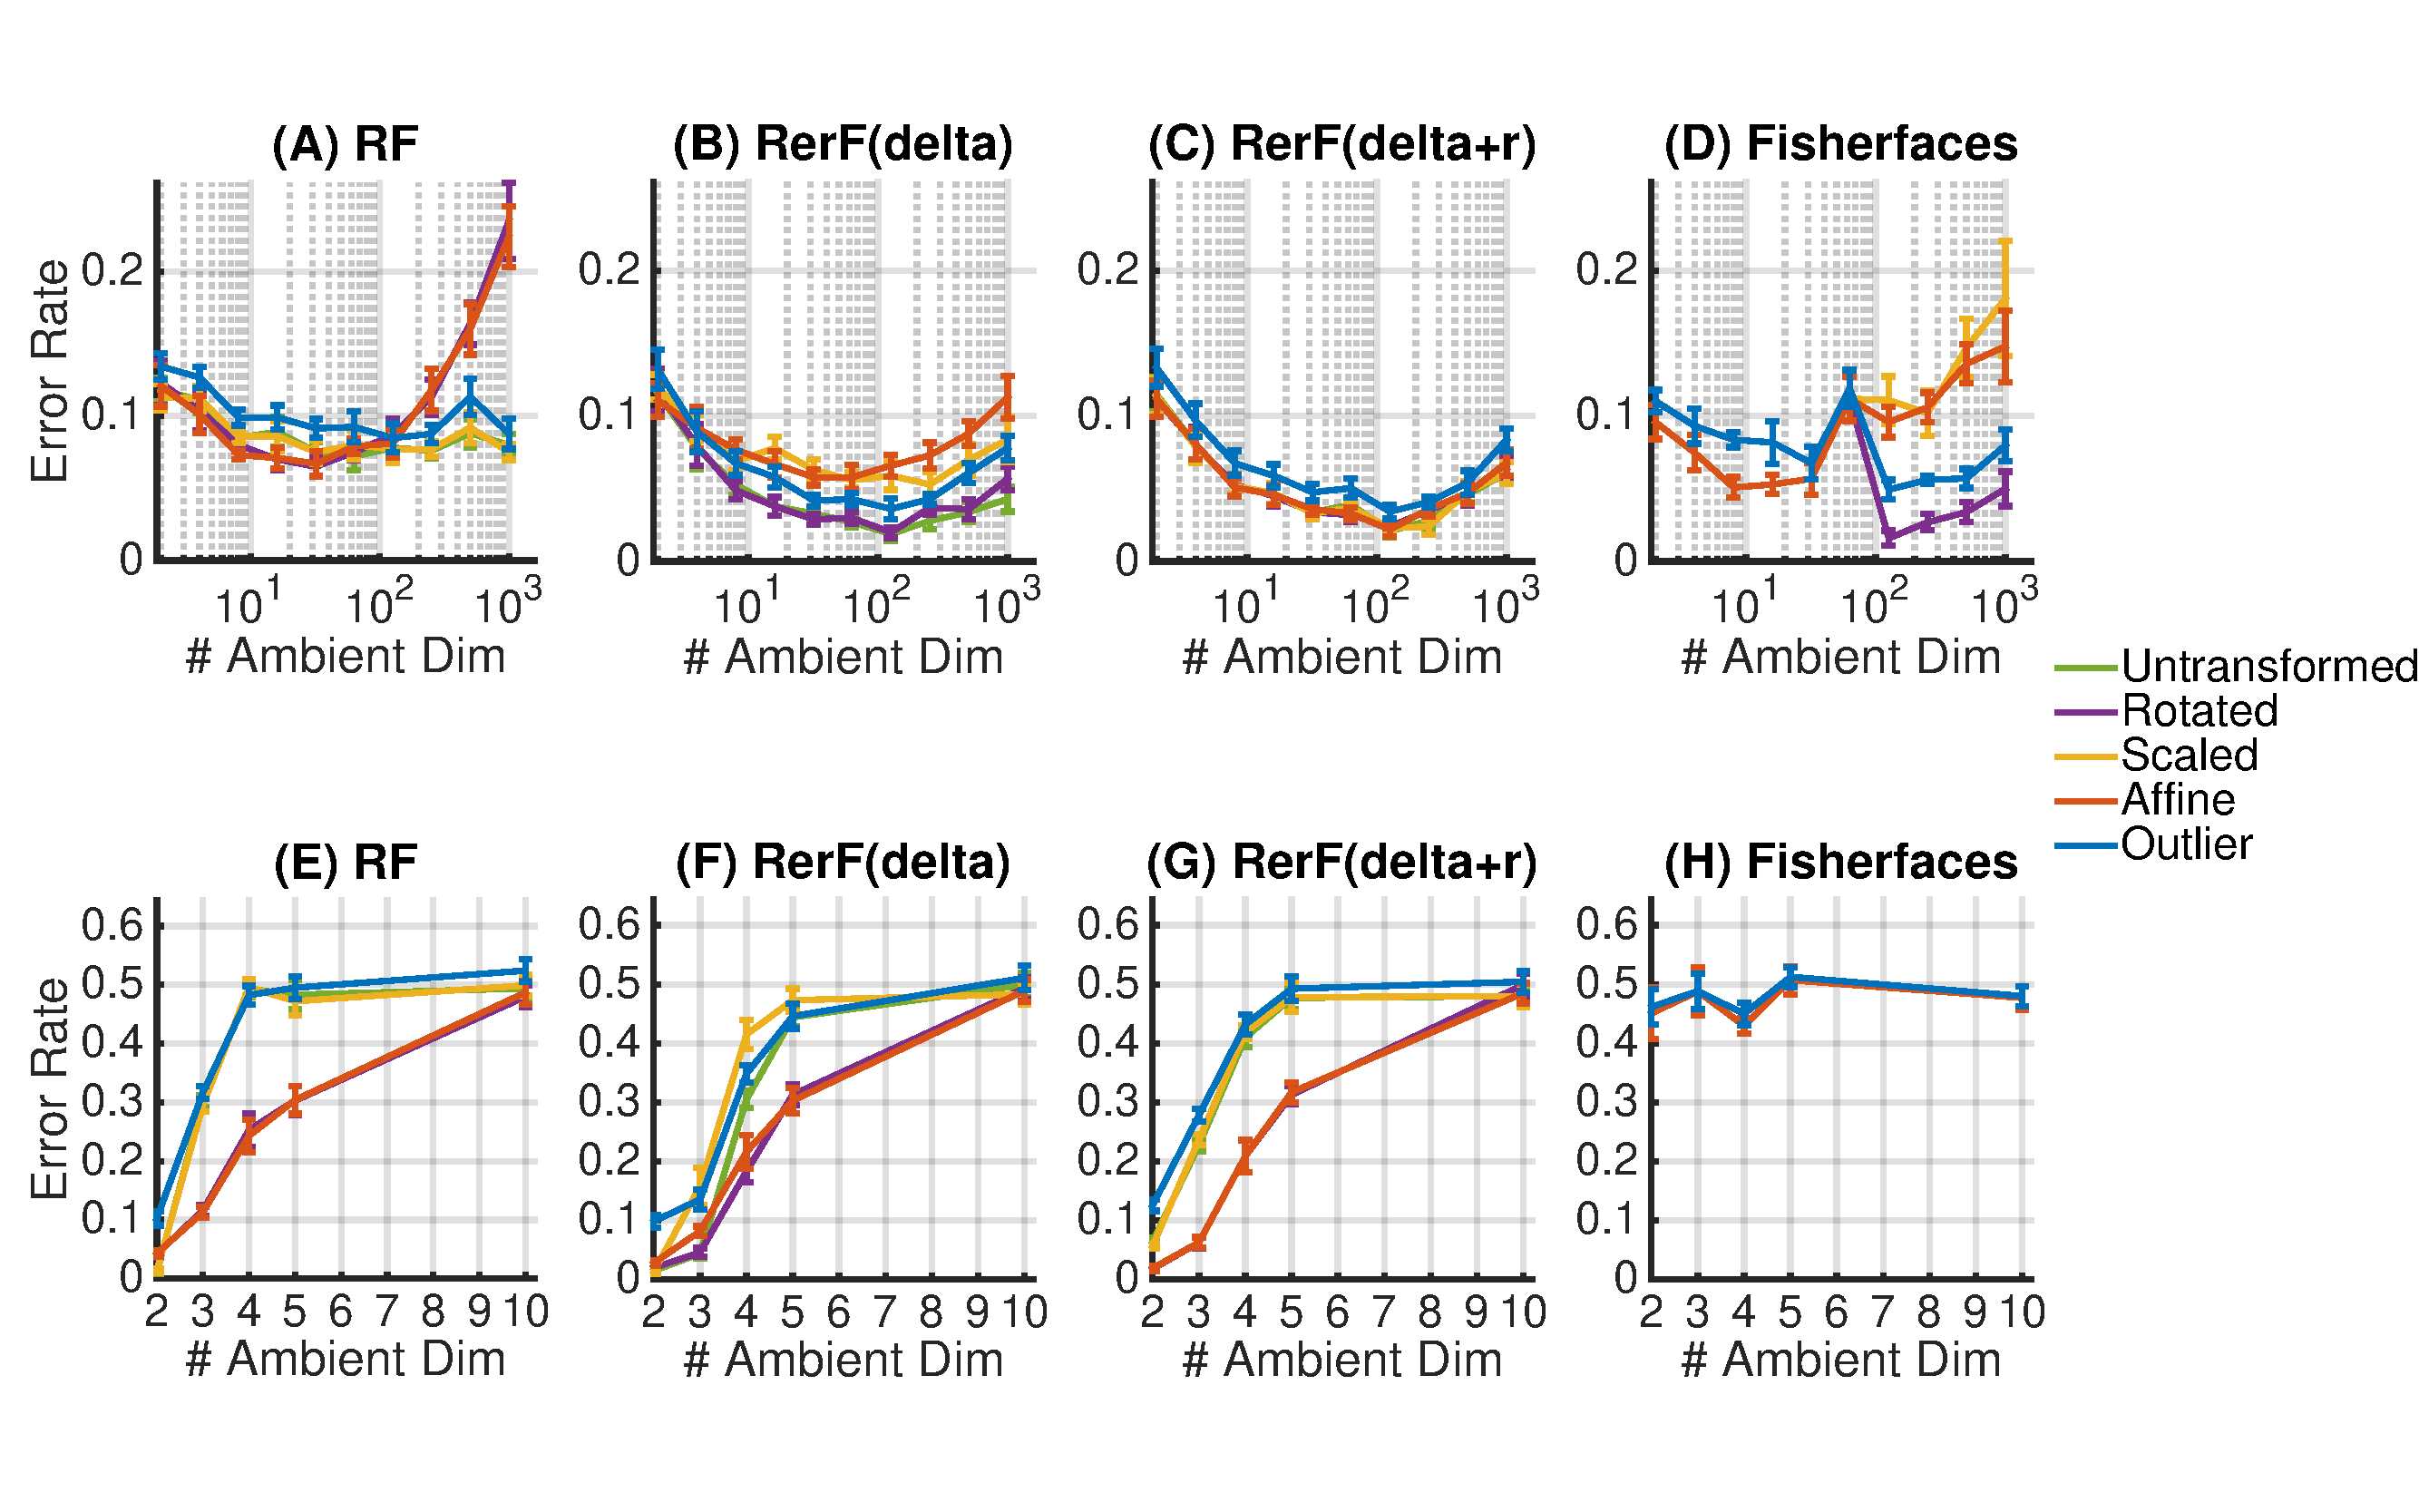
\includegraphics[trim=0in 8.75in 0in 8.75in, clip=true, width=0.8\linewidth]{Fig3_Invariance_v2}
\end{center}
\caption{}
\end{figure}

\begin{figure}[h]
\begin{center}
%\framebox[4.0in]{$\;$}
\includegraphics[trim=0in 8.75in 0in 8.75in, clip=true, width=0.8\linewidth]{Fig4}
\end{center}
\caption{}
\end{figure}

\end{document}